% !TeX spellcheck = en_US
\documentclass[sigconf,nonacm]{acmart}
\usepackage{listings}
\usepackage{caption}
\usepackage{color}
\usepackage{graphicx}
\newcounter{nalg}
\renewcommand{\thenalg}{\arabic{nalg}}
\DeclareCaptionLabelFormat{algocaption}{Algorithm \thenalg}

\lstnewenvironment{algorithm}[1][]
{
    \refstepcounter{nalg}
    \captionsetup{labelformat=algocaption,labelsep=colon}
    \lstset{
        mathescape=true,
        frame=tB,
        numbers=left,
        numberstyle=\tiny,
        basicstyle=\scriptsize,
        keywordstyle=\color{black}\bfseries\em,
        keywords={,input, output, return, datatype, function, in, true, false, if, then, else, for, to, all, do, foreach, while, begin, end, }
        numbers=left,
        xleftmargin=.04\textwidth,
        #1
    }
}
{}
\settopmatter{printacmref=false}
\pagestyle{empty}
\AtBeginDocument{%
  \providecommand\BibTeX{{%
    \normalfont B\kern-0.5em{\scshape i\kern-0.25em b}\kern-0.8em\TeX}}}
\copyrightyear{2020}
\acmYear{2020}
\setcopyright{rightsretained}
\begin{document}
\title{Group 1: Distributed Minimum Spanning Tree}
\subtitle{Prim's algorithm in C++, CUDA, CUDA Streaming and Thrust}
\author{Christian Kastner}
\email{christian.kastner@student.tuwien.ac.at}
\affiliation{Mat.Nr. 00100168}
\author{Adrian Tobisch}
\email{e1227508@student.tuwien.ac.at}
\affiliation{Mat.Nr. 01227508}
\author{Helmuth Breitenfellner}
\email{helmuth.breitenfellner@student.tuwien.ac.at}
\affiliation{Mat.Nr. 08725866}
\begin{abstract}
In this task we worked on efficient implementations of parallelized versions of Prim's
algorithm for finding the Minimum Spanning Tree using NVIDIA CUDA.
For comparison purposes, a sequential version, written in plain C++, was implemented.
Three CUDA versions were implemented, two independent implementations using plain CUDA,
and one using Thrust.
We evaluated the performance of these implementations with varying graph
densities and vertex counts. We show that the parallel implementations
suffer from a performance overhead that is noticeable with small,
sparse graphs, but that this overhead is easily amortized with larger,
and especially denser graphs. Runtime of the parallelized algorithms remained
almost constant with increasing density, while the runtime of the sequential
algorithm grew linearly.

\end{abstract}
\keywords{Prim, Minimum Spanning Tree, CUDA, C++, Thrust}
\maketitle
\section{Introduction}

In this project, we examined the potential benefits of utilizing GPU Computing in the implementation of a popular graph algorithm. Specifically, using the NVIDIA CUDA Toolkit, we implemented, in C++, three different versions of Prim’s algorithm for finding a minimum spanning tree for a graph.

We began by first creating base classes to model a graph data structure and to enable filesystem input / output. Using this base, we implemented a configurable random graph generator. We then implemented a sequential CPU version of Prim’s algorithm, for the purpose of comparison. This was followed by two independent and differing CUDA implementations, as well as one Thrust implementation. We also evaluated slight variations of these implementations, for example using CUDA Streams, Dynamic Parallelism, or different memories (paged / pinned / zero-copy). Finally, we conducted a runtime performance analysis of all of these implementations.

\section{GPU Computing and CUDA}

GPU Computing by running normal applications on graphic chips has seen a steady increase in popularity over the last few years. As single core CPU performance is reaching more and more its physical limits, multi- and many-core systems are implemented in most of today's modern IT systems. In order to utilize the full power of this ongoing evolution, the paradigm of parallel programming becomes more and more crucial for efficient computations.

Many common problems in computer science are parallelizable to a degree where the amount of parallelization is dependent on the actual problem size. In such cases the number of threads, which are able to work independently on very simple tasks at the same time, overwhelms even modern multi-core systems. For these highly parallelizable problems, graphics processing units which provide many parallel cores and very fast memory bandwidth, are the best choice. In order for developers to be able to access the graphics card by a unified interface, the leading GPU manufacturer NVIDIA released their own programming toolkit named CUDA, which will be used in this report for all experiments.

\section{Minimum Spanning Tree and Prim’s Algorithm}

The core data structure of our algorithm is the connected, weighted, undirected graph, defined by the vertices V vertices and the weighted edges E. To facilitate quantitative comparisons, we say that a graph has  n = |V| vertices and m = |E| edges.

A minimum spanning tree is a subset of the edges E such that it connects all the vertices V together, without any cycles, and with the minimum possible total edge weight [MST]. Figure 1 depicts a graph with its minimum spanning tree highlighted.


\begin{figure}
\centering
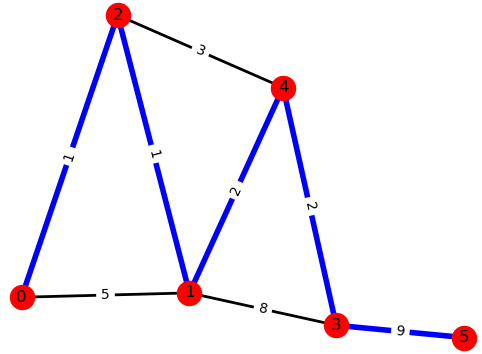
\includegraphics[width=0.7\linewidth]{graph-simple.png}
\caption{A connected, weighted, undirected graph with its minimum spanning tree highlighted in blue.}
\label{fig:graph-simple}
\end{figure}

Prim’s algorithm \cite{prim1957} is a greedy algorithm that finds such a minimum spanning tree. Starting from a single vertex, it iteratively grows by repeatedly (1) selecting all vertices that have not yet been connected to the tree, (2) finding the minimum-weight edge to any of these vertices, and (3) adding that edge to the tree, connecting the vertex.

This loop, which we term the outer loop, cannot be parallelized. However, the loops used within steps (1) and (2), which we term the inner loops, can be parallelized.

\section{Preliminaries and Baseline Implementations}


\subsection{Base Classes}

We started with implementing a base C++ class \texttt{Graph},
which encapsulates functions like file input/output, counting the edges,
and storing the graph data.
It also has a flag specifying whether the graph shall be directed or
undirected.

This base class was used as the interface for all further implementations
of Prim's algorithm.

We also tried to consistently add unit tests to all functionality,
based on the \texttt{doctest} mini-framework.

\subsection{Graph generator}

The graph generator is creating a graph, with provided size (number of vertices),
density (approximate ratio of existing vs. possible edges), and the weight range.
Also a flag can be specified whether the graph shall be directed or undirected.

\subsection{Sequential Version of Prim's Algorithm}

A  sequential version of Prim’s algorithm was implemented using a binary heap,
along the lines of the following pseudo code:
\begin{algorithm}[caption={Sequential Prim}, label={prim:cpu}]
MST-Prim(G, r):
for all v $\in$ G.V do
  in_MST[v] $\gets$ false
  distance[v] $\gets \infty$
  predecessor[v] $\gets$ null
end for
result_MST $\gets \emptyset$
in_MST[r] $\gets$ true
distance[r] $\gets$ 0
for all v $\in$ G.adj[r] do
  distance[v] $\gets$ G.weight[v,r]
  predecessor[v] $\gets$ r
end for
for i $\gets$ 1 to n-1 do
  v_next $\gets$ nearest_vertex(G, distance, in_MST)
  in_MST[v_next] $\gets$ true
  if predecessor[v_next] $\ne$ null then
    add edge(predecessor[v_next], v_next) to result_MST
  end if
  for all v $\in$ G.adj[v_next] do
    if v $\notin$ resultMST then
      if distance[v] > G.weight[v_next, v] then
        distance[v] $\gets$ G.weight[v_next, v]
        predecessor[v] $\gets$ v_next
      end if
    end if
  end for
end for
\end{algorithm}

\subsection{Boost Version of Prim’s Algorithm}

Boost is a collection of free peer-reviewed portable C++ source libraries which provides fast implementations of many common algorithms. Among these algorithms, there is a sequential implementation of Prim’s algorithm which, in our evaluations, exhibited very good performance. We selected this implementation to use as a state-of-the-art comparison baseline for our implementations.


\subsection{Evaluation Methodology}

Each algorithm was executed 1+3 times: one “warm-up” execution, where the results were discarded, and 3 regular executions. The running time for an algorithm was calculated as the mean of these regular executions.

\section{CUDA implementations of Prim’s Algorithm}

We created three parallelized implementations of Prim’s algorithm: two using pure CUDA, and one using Thrust. We also extended one of the CUDA implementation implementations to study the effects of using Dynamic Parallelism, and various memories (paged / pinned / zero-copy).

The CUDA implementations as well as the Thrust version follow the general outline of work of \cite{wang2011design}. Most notably, they also encode the original graph using compact adjacency lists, and utilize the same data structure for encoding the minimum spanning tree, building it in increments.

\subsection{Compact Adjacency List Data Structure (CAL-DS)}

The compact adjacency list as introduced by \cite{wang2011design} is a minor extension of \cite{Harish07}.
Two one-dimensional arrays of \texttt{uint2} (= 32-bit integer pairs) are allocated:
\textbf{vertices A} is of length |V|, and encodes for the vertex k where its edges can be found
in \textbf{edges B}, which is of length $2\times|E|$.\footnote{Each edge is represented twice: once for each of the two vertices it connects}.

More specifically, for any vertex k , A[k].x is the count of connected edges, and A[k].y denotes the offset of these edges in B. The first edge is therefore at B[A[k].y], and the last edge at B[A[k].y + A[k.x] - 1]. For any edge at offset o, B[o].x is ID of the other vertex,, and B[o].y is the weight of the edge.

For example, the graph of Figure 1, with 6 nodes and 8 edges, would be encoded as presented in Figure 2.

\begin{figure}
\centering
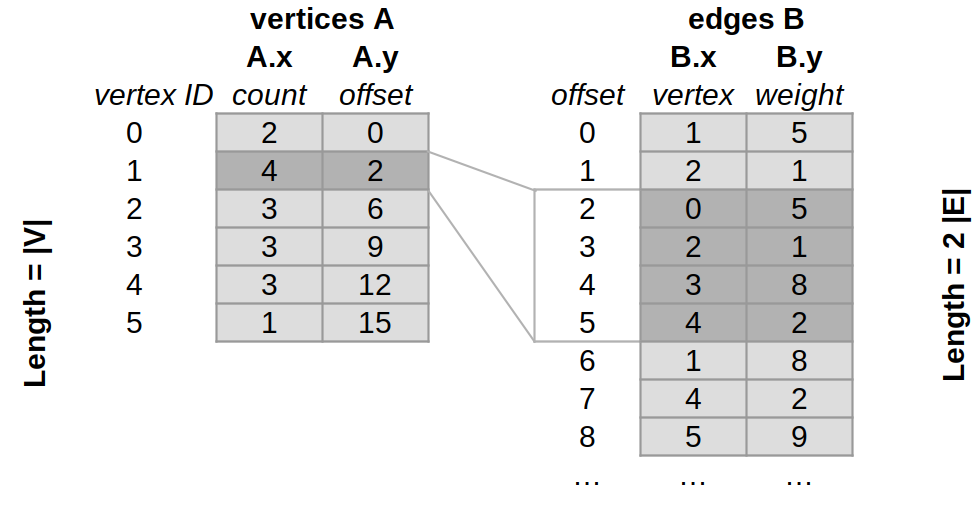
\includegraphics[width=0.7\linewidth]{compact-adjacency-list.png}
\caption{Compact adjacency list representation for the graph of Figure Y. The highlighted vertex with ID=1 has 4 outgoing edges, the data of which is stored beginning at offset 2.}
\label{fig:compact-adjacency-list}
\end{figure}

\subsection{Minimum Spanning Tree Data Structure (MST-DS)}

The minimum spanning tree is encoded with the data structure used by [Wang11], consisting of three one-dimensional arrays of length |V|-1, one for each property of the |V|-1 edges of a minimum spanning tree: outgoing vertex, incoming vertex, and weight. The data structure for the minimum spanning tree of the graph in Figure 1 is visualized in Figure 3.

\begin{figure}
\centering
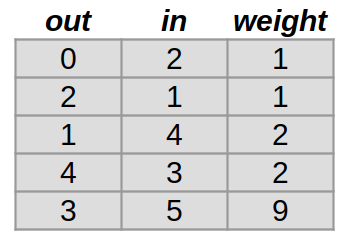
\includegraphics[width=0.7\linewidth]{mst-datastructure}
\caption{MST-DS for the minimum spanning tree for the graph in Figure 1.}
\label{fig:mst-datastructure}
\end{figure}

It is important to note that this data structure is not used merely to encode the final result. Instead, it is created at the very beginning using an initial state, and then used to incrementally and efficiently build the final result in-place.


\subsection{General Outline of the Algorithm}

The algorithm begins by initializing the CAL-DS and MST-DS as described above.

The CPU drives the execution through the outer loop of Prim’s algorithm. The inner loop of the algorithm generally consists of executing CUDA kernels for each of the following primitives:

\begin{enumerate}
\item \textbf{Update} the weights in the MST-DS. For every vertex P in the inbound list not yet included in the MST, if there exists an edge from the current vertex C to this vertex P with a weight better than the currently known best, update the entry for vertex P.
$\rightarrow$ This step can be parallelized
\item \textbf{Find} the minimum weighted edge in the MST-DS
$\rightarrow$ This is the core step and can also be parallelized in the form of a Min-Reduction. For non-trivial graphs, Min-Reduction generally involves two kernel invocations:
The first kernel takes the input edges and loads them into blocks, computes the  block minimum, and stores each block minimum in shared memory
The second kernel takes the block minima from shared memory, and reduces them to a global minimum.
\item \textbf{Pick} this newly found minimum-weighted edge, and designate its inbound vertex to be the new C.
\end{enumerate}

These three steps are repeated until every vertex has been included in the MST. Figure 4 visualizes these steps in a workflow fashion.

\subsection{CUDA - Implementation \#1 (CUDA1)}

The first algorithm approach inherits many implementation principles from the paper and is a multi-kernel solution. The Cuda-Multi implementation calls four different cuda kernels in a loop in order to update new paths, find the best-fitting edge and update the solution by each new node found. All four kernels assemble into a cycle of prim’s algorithm and is called exactly V-1 times where V is the number of vertices of the input graph.

Starting with the setup phase of the algorithm there are four different components which are set up in order to run the application.

\begin{enumerate}
\item $\underline{\textrm{vertices, edges}}$\\
These arrays represent the input graph as CAL-DS as described above.

\item $\underline{\textrm{inbound, outbound, weights}}$\\
These three arrays represent the mst-solution and are already referred as MST-DS above. Differently to the paper’s implementation this algorithm initializes each array with length |V| instead of |V-1|. This adjustment was implemented due to the changed indexing during the update-step and will be further described later on.

\item $\underline{\textrm{current\_node, last\_node}}$\\
In addition to the current node, which is already used in the paper the last node is also stored in an extra variable.

\item $\underline{\textrm{v\_red}}$\\
v\_red is a temporary array which is used to move local solutions from the first reduction step into the second kernel to avoid global synchronization costs for direct blockwise reduction.

\end{enumerate}

After the initialization phase of all previous components a function for calculating an optimized block and thread count is called. As for modern NVIDIA GPUs 32 threads are grouped into wards and then executed on the chip. Further experiments have shown that high thread counts also degrade the performance of the algorithm, and therefore avoided by the calculation. Currently, thread and block counts are defined as

\begin{tabular}{|l|l|l|}
\hline
Number of Vertices & Block Count & Thread Count \\
\hline
2 - 8192 & $2^{\lceil log_2(\frac{V}{32})}$ & 32 \\
\hline
8193 - 16384 & $2^{\lceil log_2(\frac{V}{128})}$ & 128 \\
\hline
16385 - 131072 & $2^{\lceil log_2(\frac{V}{512})}$ & 512 \\
\hline
> 131072 & $2^{\lceil log_2(\frac{V}{1024})}$ & 1024 \\
\hline
\end{tabular}

As already stated, before the actual cuda part of the algorithm consists of four kernels which form two alternating phases.

The first step of the algorithm is the update-path step where all edges from reachable nodes outgoing from the current node are compared to the already found best current edges for each inbound node. If the new connection’s weight is less than the current best then it is replaced. Each thread compares exactly one edge at a different index; therefore, this step is well suited for parallelization.

In the next step all possible solutions are read into a shared memory and min-reduction is performed. To avoid global memory accesses minimal solutions for each block are stored in a memory v\_red. In order to avoid bank conflicts as much as possible each thread processes neighboring array indices at the same time.

In the second min-reduction kernel all partial solutions in v\_red are reduced again and stored in v\_red[0]. For large problems where the number of blocks is higher than the number of threads one thread must perform more than one reduction in an iteration but the memory access strategy is the same as in the previous step. In the end, current\_node is stored in last\_node and the best global solution v\_red[0] is the new current\_node.

Lastly there is the update-edge step where the newfound edge is added into the solution arrays. In order to not overwrite already valid solutions, the best node uses last\_node as index in outbound, inbound and weights because last\_node can never occur twice during one execution of the algorithm. For that reason, this step can be performed really fast.


\subsection{CUDA - Implementation \#2 (CUDA2)}


This implementation attempted to follow the approach of \cite{wang2011design} as closely as possible. The general algorithm is just as described in the General Outline above.

\cite{wang2011design} added a particular approvement to the general approach: when incrementally building the result, the MST-DS is split into two sets: The set of edges that have already been permanently selected for inclusion in the MST, and the set of remaining “candidate” edges -- one edge for each of the vertices to which a path does not yet exist. In each iteration, after the candidate edge list has been updated, the best candidate edge is locked in by moving it from the candidates list to the permanent list.

The advantage of this approach is that the number of edges that must be updated and evaluated in each iteration continuously decreases, thereby continuously reducing the number of memory operations required.

This implementation uses the Update / Find / Pick primitives as presented in the General Outline, with the following modifications:
\begin{itemize}
\item Each kernel is invoked with memory pointing to the remaining “candidate” data instead of all the data
\item The Pick primitive moves (via a swap operation) the best edge to the beginning of the remaining “candidate” list, if the edge is not already there
\item After each iteration, the window of “candidate” data is reduced by 1, thereby locking in the edge just picked into the MST.
\item The MST-DS is extended with a fourth array v2i\_map of length |V|-1.  It tracks the current position of any incoming vertex in the MST-DS, which can move whenever edges are swapped. Using this additional information, the UPDATE primitive can reduce its work to only a few candidate edges, rather than having to full-scan all remaining candidates. This dramatically improved performance of the algorithm.
\item The implementation contains parameters with which the memory handling can be specified (paged / pinned / zero-copy).
\end{itemize}


Before the algorithm commences its first iteration, the MST-DS is initialized with all theoretically possible |V|-1 edges from some arbitrary initial vertex C, which we always chose to be the vertex 0. All edges are initially set to an edge weight of infinity.

For example, for the graph in Figure 1 with 6 vertices, the initial state of the MST-DS is given in Figure 6, and Figure 7 presents two iterations of applying the three primitives.

\begin{figure}
\centering
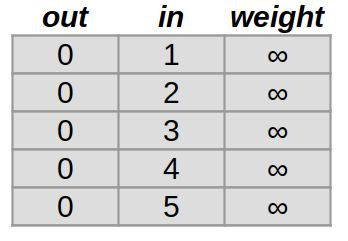
\includegraphics[width=0.7\linewidth]{mst-datastructure-initial}
\caption{MST-DS for the minimum spanning tree for the graph in Figure Y}
\label{fig:mst-datastructure-initial}
\end{figure}

\begin{figure}
\centering
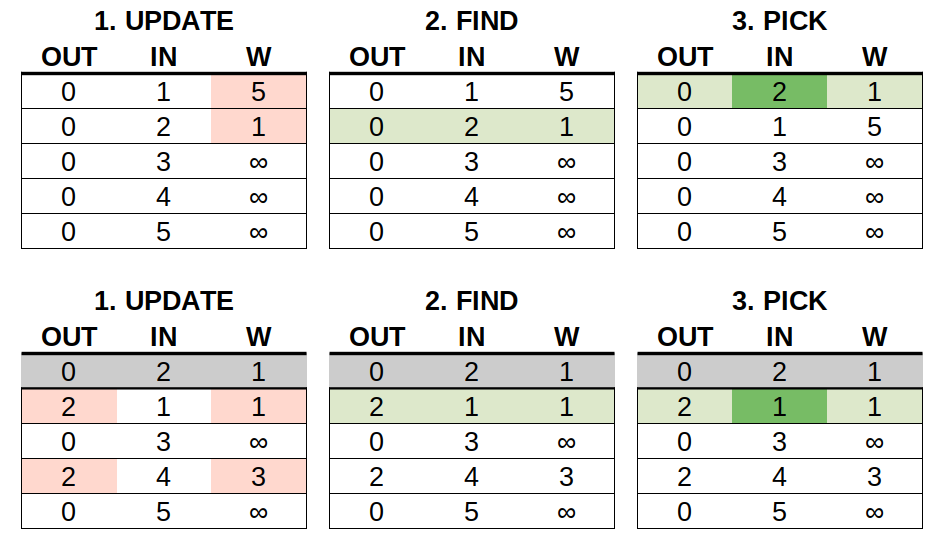
\includegraphics[width=0.7\linewidth]{algo}
\caption{Two iterations of the CUDA2 implementation.The initial state of the MST-DS is that of Figure 6. First iteration, five candidate edges remain. UPDATE: From vertex C=0, the graph contains two candidate edges, to vertices 1 and 2. Their weights are better than the previously known ones, so they are updated (red). FIND: The best edge is in the second row (green). PICK: The best edge is moved to the first row, and its inbound vertex 2 (dark green) becomes the new C. Second iteration: the first row has been locked in (grey), only four candidates remain now. UPDATE: From vertex C=2, the graph contains two candidate edges, to vertices 1 and 4. (The third edge from C=2, to vertex 0, is not in the candidate list. A path to 0 already exists). FIND: The best edge is already in the first row (green). PICK: The best edge is already at the beginning, no moving needed. Its inbound vertex 1 becomes the new C.}
\label{fig:algo}
\end{figure}

\subsection{Thrust Implementation}

The implementation of Prim's algorithm using the Thrust library follows again the general concept of [Wang11]. It uses Thrust sequences for the initialization, the Thrust min-reduction, and two regular CUDA kernels for the Update and Pick steps. For both steps we did not find an efficient way to implement them only using Thrust, therefore we used CUDA kernels for this.

In preparation of the execution a setup is called, which copies the graph into two into \texttt{thrust::device\_vector<uint2>}
objects. Their structure is identical to what has been used in the CUDA implementations. Using Thrust counting iterators, the resulting MST is initialized to a graph from the start vertex (again using vertex with the number 0) to all other vertices, with a weight of infinity.

The first step called is the update-step, using a CUDA kernel. Here the edges from vertex 0 are used to update the weights in the skeleton MST.
Then the algorithm uses a loop, going from 0 to V-1. The loop variable is used for indicating the barrier between finished and still pending vertices in the MST. In the loop using Thrust min-reduction it looks for the minimum weight in the still pending part of the MST. The minimum position will then be swapped with the position indicated by the loop variable, using again a CUDA kernel. The CUDA kernel is used to avoid unnecessary copying between host and device for a simple swap operation. Following that is a call to the update operation.

The update operation has a slightly different behavior depending on whether it is called for the first iteration or if it is called within the loop. In the first call, the barrier is set to 0, meaning that the current node has the number 0. In the calls in the loop, the barrier variable is set to the loop variable, incremented by 1. This causes the kernel to take the last vertex in the MST before the barrier as the starting node for updating the edge weights.

At the end the resulting MST is copied from device memory back to host memory for the caller.

\section{Evaluation}

\subsection{Experimental Setup}


The main batch of experiments were carried out on a host with a 4-core Intel i7-3770 Ivy Bridge CPU, 16GB of DDR3 RAM, and an MSI GTX 1650  (Turing) graphics card attached via PCIe 3.0. The operating system was Debian Linux 10.4 (“buster”), and the NVIDIA CUDA Toolkit version was 1.0.243.

\subsection{Effects of density}

The measure the effects of the density of a graph on the implementations’ performances, we executed them constant vertex counts,|V|=4096 and |V|=8192, and with densities 0.01, 0.05, 0.1, 0.3, 0.5, 0.7, and 1.0.

Figures 8 and 9 visualize the runtimes of the individual algorithms with these settings.

By comparison to the sequential Boost implementation, it is evident that the parallel implementations have an overhead cost that is present regardless of the graph density.

But while with increasing density, Boost’s runtime increased almost linearly, the runtime curves of the parallelized implementations remained almost flat, suggesting that given a sufficiently dense graph, Prim’s algorithm can indeed tremendously benefit from GPU computing.

\subsection{Effects of Vertex Count}

\subsection{Effects of Memories}

We also evaluated the CUDA2 implementation  using different memory access patterns, namely regular (paged) memory, pinned memory, and zero-copy memory (= all memory allocations on the host, and mapped to device memory space)

From the results, we conclude the following:
\begin{itemize}
\item For non-trivial graphs, pinning memory had a noticeable positive effect on memory transfer performance, which improved with growing graph size. It is our understanding that when using paged memory, CUDA must transfer the data to pinned memory before it can be transferred to the device, so allocating pinned memory from the beginning removes one memory copy step from the process.
\item Unsurprisingly, using zero-copy memory for all operations (no device memory allocation!) had a noticeable negative effect on overall performance. However, that negative effect increased at most linearly with test difficulty, suggesting that the GPU might be performing some effective caching.
\end{itemize}

\subsection{CUDA1 vs CUDA2}

\section{Conclusions}

Our main conclusion is that given a sufficiently dense graph, Prim’s algorithm can indeed tremendously benefit from GPU computing, despite the fact that the algorithm itself has a sequential characteristic, and is only partially parallelizable.

Furthermore, we made the following notable observations:
\begin{itemize}
\item Launching a CUDA kernel to update a value is faster than memory transfer\\
During the evolution of our implementation, it became necessary to update a single 32-bit integer in CUDA memory. We assumed that D2H-updateOnHost-H2D would be faster than launching a kernel to do the update on the GPU, but experiments proved us wrong -- launching a kernel is actually faster.

\item Dynamic Parallelism can be faster, but requires the right workloads\\
Especially in the CUDA2 implementation with its continuously reducing workload, Dynamic Parallelism, where we used a “parent” kernel to distribute workloads to “child” kernels, did not bring major benefits, and in fact was slower than the non-dynamic approach.

\item Prioritize simple solutions during early implementation phases\\
Keeping an algorithm suited for evolution during the implementation turned out to be a major benefit for CUDA2. Since CUDA1 was optimized for quick updates by a special indexing system, later observed flaws were too difficult to fix without bringing more boilerplate code to it. Therefore, the reduction-phase became the weak spot of the whole implementation, which resulted in performance fluctuations for certain inputs.

\item CUDA Streams was not applicable\\
We evaluated whether we could utilize CUDA Streams, but unfortunately that was not possible. The algorithm requires the entire data to be present in memory before the first iteration begins. Hence, it was not possible to benefit from streaming data.

\end{itemize}


\bibliographystyle{ACM-Reference-Format}
\bibliography{report}
\end{document}
